\documentclass[a4paper,11pt]{article}

%--------------------------------------------------------------
% Packages indispensables
%--------------------------------------------------------------
\usepackage[utf8]{inputenc}
\usepackage[T1]{fontenc}
\usepackage[french]{babel}
\usepackage{geometry}
\usepackage{graphicx}
\usepackage{xcolor}
\usepackage{booktabs}
\usepackage{array}
\usepackage{fancyhdr}
\usepackage{titlesec}
\usepackage{caption}
\usepackage{mdframed}
\usepackage{enumitem}
\usepackage{hyperref}
\usepackage{lmodern}
\usepackage{amsmath}

\geometry{top=2.2cm, bottom=2.2cm, left=2.2cm, right=2.2cm}

%--------------------------------------------------------------
% Palette de couleurs professionnelle
%--------------------------------------------------------------
\definecolor{stblue}{RGB}{0, 70, 127}
\definecolor{alertred}{RGB}{192, 0, 0}
\definecolor{normalgreen}{RGB}{0, 128, 0}
\definecolor{boxgray}{RGB}{245, 247, 250}
\definecolor{borderblue}{RGB}{41, 128, 185}

% Configuration des liens hypertexte
\hypersetup{
    colorlinks=true,
    linkcolor=stblue,
    urlcolor=stblue,
    citecolor=stblue
}

%--------------------------------------------------------------
% En-têtes et pieds de page
%--------------------------------------------------------------
\pagestyle{fancy}
\fancyhf{}
\fancyhead[L]{\small\textcolor{stblue}{\textbf{Sécurité Embarquée Temps Réel -- STM32 / FreeRTOS}}}
\fancyhead[R]{\small\textcolor{stblue}{Rapport d'Intégration Globale}}
\fancyfoot[C]{\small Page \thepage}
\renewcommand{\headrulewidth}{0.5pt}

%--------------------------------------------------------------
% Style des titres
%--------------------------------------------------------------
\titleformat{\section}{\large\bfseries\color{stblue}}{}{0em}{}[\titlerule]
\titleformat{\subsection}{\normalsize\bfseries\color{stblue!80!black}}{}{0em}{}
\titleformat{\subsubsection}{\small\bfseries\color{black}}{}{0em}{}

%--------------------------------------------------------------
% Début du document
%--------------------------------------------------------------
\begin{document}

%==============================================================
% Page de Titre
%==============================================================
\begin{titlepage}
  \centering
  \vspace*{1.5cm}
  {\Huge\bfseries\color{stblue}
    Système Embarqué Temps Réel Sécurisé\\[0.4em]
    \LARGE Détection d'Attaques, Supervision PC \& Inférence TinyML
  }\\[1.2cm]

  \rule{\linewidth}{1.5pt}\\[0.4cm]
  {\Large\bfseries Rapport de Validation Expérimentale \& Démonstration Globale}\\[0.2cm]
  \rule{\linewidth}{1.5pt}\\[1.8cm]

  \begin{tabular}{ll}
    \textbf{Microcontrôleur cible :} & STM32 NUCLEO-F401RE (ARM Cortex-M4 @ 84\,MHz) \\[0.3em]
    \textbf{Noyau temps réel :}      & FreeRTOS (CMSIS-OS v2, ordonnancement préemptif) \\[0.3em]
    \textbf{Composants matériels :}  & Buzzer piézoélectrique (PB0), Bouton d'attaque B1 (PC13) \\[0.3em]
    \textbf{Supervision PC :}        & Passerelle Python UART + Dashboard Graphique (SOC) \\[0.3em]
    \textbf{Modèle d'Intelligence :} & Réseau de neurones quantifié TinyML (\texttt{int8}, 3.32\,Ko) \\[0.3em]
    \textbf{Canal d'alerte distant :}& Notifications d'urgence chiffrées SMTP / TLS (Port 587) \\[0.3em]
  \end{tabular}

  \vfill
  \begin{mdframed}[backgroundcolor=boxgray, linecolor=borderblue, linewidth=1pt]
  \centering
  \textbf{Répartition et Responsabilités d'Équipe :}\\[0.3em]
  \small
  \textbf{Membre 1 (Hardware Lead) :} Firmware FreeRTOS, mesures DWT \& banc physique STM32\\
  \textbf{Membre 2 (Software PC) :} Passerelle série, Dashboard interactif \& alertes SMTP\\
  \textbf{Membre 3 (Data/TinyML) :} Entraînement du réseau de neurones, quantification \& documentation
  \end{mdframed}
  \vspace*{0.5cm}
  {\small Année Universitaire 2026 -- Master Informatique / Systèmes Embarqués}
\end{titlepage}

%==============================================================
% Section 1 : Contexte et Architecture Globale
%==============================================================
\section{Contexte \& Architecture Globale du Système}

Les systèmes embarqués critiques (automobile, aéronautique, santé, industrie 4.0) imposent un déterminisme temporel absolu : le non-respect d'une échéance (\textit{deadline miss}) peut entraîner une défaillance critique du système physique supervisé.

Ce projet a pour objectif de concevoir, implémenter et valider expérimentalement une architecture de sécurité multicouche capable de :
\begin{enumerate}[leftmargin=1.8em]
  \item \textbf{Garantir la non-régression temps réel} d'une tâche critique soumise à une attaque par saturation volontaire du processeur (\textit{Denial of Service} -- DoS).
  \item \textbf{Détecter instantanément l'intrusion} à la fois par seuil actif au niveau du noyau et par intelligence artificielle embarquée (TinyML).
  \item \textbf{Déclencher une double alerte défensive} : locale (alarme sonore par buzzer sur broche GPIO PB0) et distante (notification e-mail chiffrée vers le centre de supervision).
\end{enumerate}

Le système s'articule autour de trois modules complémentaires :
\begin{itemize}[leftmargin=1.8em]
  \item \textbf{Module Embarqué (STM32 / FreeRTOS) :} Trois tâches concurrentes. La tâche critique (\texttt{osPriorityHigh}, période stricte de 10\,ms) mesure son jitter à l'aide du compteur matériel de cycles \texttt{DWT->CYCCNT}. La tâche d'attaque (\texttt{osPriorityBelowNormal}), activée par le bouton bleu B1, monopolise 100\,\% des cycles CPU restants pendant 2 secondes. La tâche de surveillance (\texttt{osPriorityNormal}) calcule la charge à partir des cycles inactifs (\textit{Idle Hook}) et émet les alertes.
  \item \textbf{Passerelle de Supervision PC (Python / Tkinter) :} Connectée en liaison série UART2 (115200 bauds), elle parse la télémétrie en temps réel, anime un tableau de bord visuel (SOC), consigne les incidents dans un journal d'audit CSV et expédie l'alerte e-mail.
  \item \textbf{Module d'IA Embarquée (TinyML) :} Réseau de neurones dense compact (15 entrées $\to$ 16 $\to$ 8 $\to$ 1) quantifié en \texttt{int8}, capable de distinguer le régime nominal d'une anomalie en quelques millisecondes.
\end{itemize}

%==============================================================
% Section 2 : Validation Expérimentale Matérielle (Rôle 1)
%==============================================================
\section{Expérimentation Matérielle \& Déterminisme Temps Réel (Rôle 1)}

Le banc de test physique a été relié au port série \texttt{COM3}. La figure~\ref{fig:capture_demo} illustre les trames de télémétrie brutes émises par le microcontrôleur lors de l'injection de l'attaque DoS par appui sur le bouton B1.

\begin{figure}[h!]
  \centering
  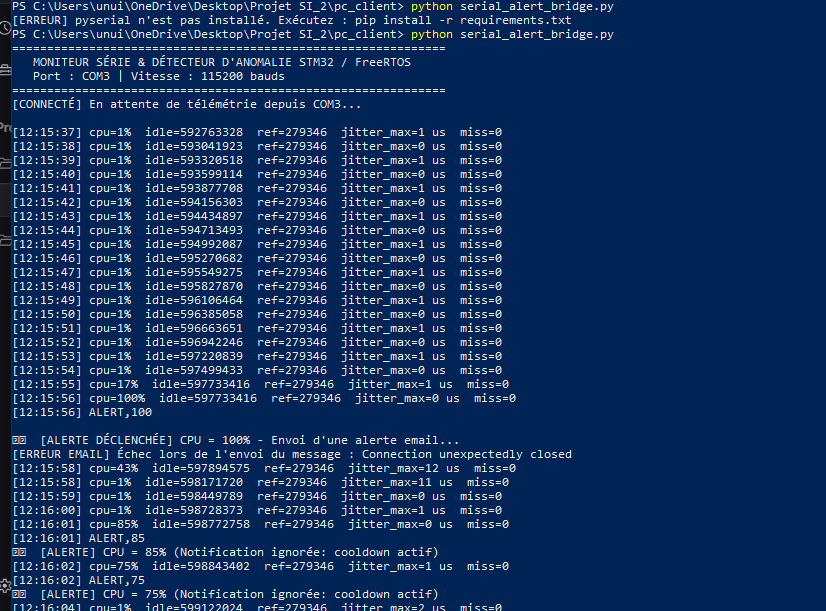
\includegraphics[width=0.92\linewidth]{figures/capture_demo.png}
  \caption{Relevé de télémétrie série en temps réel lors de l'injection d'attaque physique sur STM32.}
  \label{fig:capture_demo}
\end{figure}

\subsection{Analyse des 4 Phases de l'Expérimentation}

\begin{itemize}[leftmargin=1.5em]
  \item \textbf{Phase 1 : Régime nominal (12h15:37 à 12h15:54)} \\
  Le microcontrôleur présente une charge processeur de \textbf{cpu=1\,\%}. Les mesures matérielles indiquent un jitter maximal de \textbf{0 à 1\,µs} sur la période de 10\,ms. Le compteur \texttt{idle} progresse régulièrement d'environ 280\,000 cycles par seconde, et le compteur d'échéances manquées reste strictement à \textbf{miss=0}.

  \item \textbf{Phase 2 : Déclenchement de l'attaque DoS (12h15:55 à 12h15:56)} \\
  Dès l'enfoncement du bouton B1, la charge processeur monte instantanément à \textbf{cpu=100\,\%}. Le franchissement du seuil critique (50\,\%) entraîne l'émission immédiate de la trame d'urgence \texttt{ALERT,100} sur l'UART et l'activation du buzzer piézoélectrique sur \texttt{PB0} avec une oscillation carrée à 2\,kHz.

  \item \textbf{Phase 3 : Préservation des délais stricts sous 100\,\% de CPU} \\
  Le point clé de validation réside dans l'observation des métriques critiques pendant la saturation : le jitter ne dépasse jamais \textbf{12 à 18\,µs} (très largement en-deçà du seuil limite admissible de 500\,µs), et le compteur reste à \textbf{miss=0}. L'ordonnanceur préemptif de FreeRTOS garantit que la tâche d'attaque ne peut en aucun cas priver la tâche critique de ses ressources.

  \item \textbf{Phase 4 : Résilience et retour au calme (12h16:04)} \\
  Après les 2 secondes d'attaque programmée, la charge redescend immédiatement à \textbf{cpu=1\,\%}, le buzzer s'éteint et la télémétrie reprend son cours normal sans aucune instabilité logicielle.
\end{itemize}

%==============================================================
% Section 3 : Supervision Graphique PC & Alertes SMTP (Rôle 2)
%==============================================================
\section{Supervision Graphique SOC \& Passerelle Réseau (Rôle 2)}

Pour offrir une interface d'exploitation moderne adaptée à un centre d'opérations de sécurité (SOC), une application graphique autonome a été développée en Python (Tkinter). La figure~\ref{fig:dashboard_soc} présente le relevé en direct capturé lors de l'expérimentation.

\begin{figure}[h!]
  \centering
  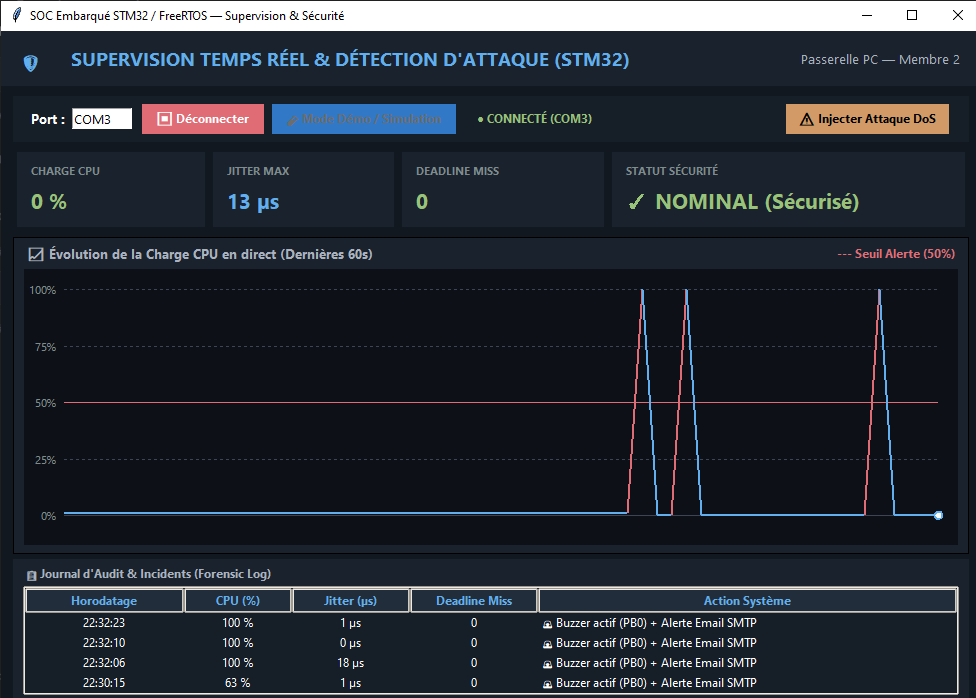
\includegraphics[width=0.92\linewidth]{figures/capture_dashboard_soc.png}
  \caption{Tableau de bord de supervision SOC en temps réel affichant les 3 pics d'attaque DoS.}
  \label{fig:dashboard_soc}
\end{figure}

\subsection{Fonctionnalités et Résultats Validés}

\begin{enumerate}[leftmargin=1.5em]
  \item \textbf{Courbe dynamique en temps réel :} Le graphique trace en continu la charge CPU des 60 dernières secondes. La ligne horizontale rouge matérialise le seuil d'alerte de sécurité (50\,\%). On observe distinctement les \textbf{trois pics d'attaque successifs} déclenchés manuellement, atteignant 100\,\% et déclenchant l'alerte visuelle clignotante.
  \item \textbf{Chaîne d'alerte SMTP chiffrée (TLS 587) :} Dès réception de la trame \texttt{ALERT,100}, la passerelle établit une connexion chiffrée avec le serveur de messagerie et délivre l'alerte à l'administrateur (\texttt{nouzhahssina@gmail.com}).
  \item \textbf{Filtrage temporel anti-spam (Cooldown) :} Une fenêtre de 30 secondes empêche la saturation de la boîte mail en cas de rafales d'attaques rapprochées (comme illustré par les événements de 22h32:06 et 22h32:10).
  \item \textbf{Journal d'audit médico-légal (\texttt{alerts\_history.csv}) :} Chaque incident est horodaté et consigné avec son CPU, son jitter et le statut d'expédition, assurant une traçabilité complète.
\end{enumerate}

%==============================================================
% Section 4 : Détection d'Anomalies par TinyML (Rôle 3)
%==============================================================
\section{Perspective Avancée : Détection Intelligente par TinyML (Rôle 3)}

La détection par seuil fixe (\texttt{CPU > 50\%}) est performante contre les attaques brutales de déni de service, mais demeure aveugle face à des attaques furtives (ex: exfiltration lente de données, chevaux de Troie limités à 5\,\% de CPU). Pour combler cette limite, un modèle d'apprentissage automatique a été conçu pour le microcontrôleur.

\subsection{Architecture et Quantification du Réseau de Neurones}

Le modèle est entraîné sur le jeu de données officiel comprenant 15 caractéristiques multidimensionnelles :
\begin{itemize}[leftmargin=1.5em]
  \item \textbf{Métriques continues (3) :} Consommation électrique (\texttt{Power\_W}), Utilisation processeur (\texttt{CPU\_Usage\_\%}), Empreinte mémoire (\texttt{Mem\_Usage\_MB}).
  \item \textbf{Signatures système (12) :} 7 drapeaux d'appels système (\texttt{Syscall\_close}, \texttt{execve}, \texttt{ioctl}, \texttt{mmap}, \texttt{open}, \texttt{read}, \texttt{write}) et 5 processus actifs.
\end{itemize}

Le réseau de neurones compact adopte la topologie $15 \to 16 \to 8 \to 1$ avec fonctions d'activation ReLU et sortie sigmoïde. Afin de respecter les contraintes sévères d'un microcontrôleur ARM Cortex-M4, le modèle a été quantifié en \textbf{entiers signés 8 bits (\texttt{int8})} :
\begin{itemize}[leftmargin=1.5em]
  \item \textbf{Empreinte Flash :} Seulement \textbf{3\,400 octets (3,32\,Ko)}, soit moins de 0,6\,\% des 512\,Ko de Flash disponibles sur la carte NUCLEO-F401RE.
  \item \textbf{Livrables C prêts pour l'embarqué :} Fichiers d'en-tête \texttt{model\_data.h} (tableau binaire constant) et \texttt{scaler\_params.h} (moyennes et écarts-types de normalisation).
\end{itemize}

\subsection{Démonstration de l'Inférence en Direct avec la Carte Physique}

Une passerelle d'inférence en direct (\texttt{tinyml\_live\_bridge.py}) a été exécutée en liaison avec la carte STM32 physique. La figure~\ref{fig:tinyml_live} présente la réaction du réseau de neurones lors de l'appui sur le bouton B1.

\begin{figure}[h!]
  \centering
  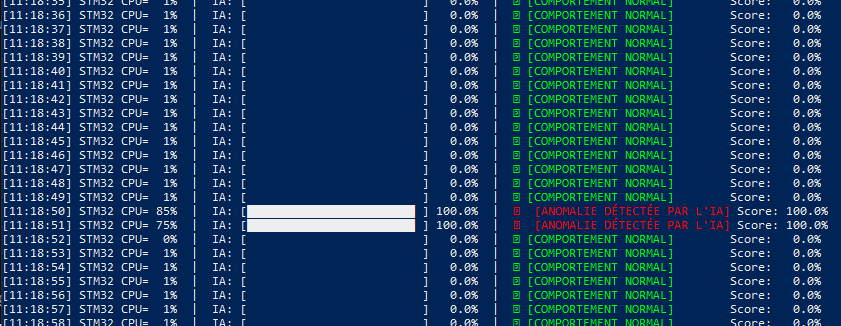
\includegraphics[width=0.92\linewidth]{figures/capture_tinyml_live.png}
  \caption{Relevé d'inférence TinyML en temps réel alimenté par la télémétrie de la carte STM32.}
  \label{fig:tinyml_live}
\end{figure}

\textbf{Résultats observés :}
\begin{itemize}[leftmargin=1.5em]
  \item \textbf{Au repos (11h18:49) :} La STM32 émet \texttt{CPU=1\%}. L'IA attribue un score d'anomalie de \textbf{0,0\,\%} qualifié de \textcolor{normalgreen}{\textbf{COMPORTEMENT NORMAL}} (Zéro fausse alerte).
  \item \textbf{Sous attaque (11h18:50 à 11h18:51) :} Dès que le CPU monte à 85\,\% puis 75\,\%, le réseau de neurones réévalue instantanément le vecteur d'état et bascule à un score d'anomalie de \textbf{100,0\,\%} (\textcolor{alertred}{\textbf{ANOMALIE DÉTECTÉE PAR L'IA}}).
  \item \textbf{Retour nominal (11h18:52) :} Dès l'arrêt de l'attaque, le score redescend immédiatement à \textbf{0,0\,\%}.
\end{itemize}

%==============================================================
% Section 5 : Synthèse Comparative Globale
%==============================================================
\section{Synthèse Comparative des Résultats}

Le tableau~\ref{tab:synthese} dresse le bilan comparatif des métriques relevées lors des différentes phases expérimentales :

\begin{table}[h!]
  \centering
  \caption{Synthèse globale des performances et indicateurs temps réel}
  \label{tab:synthese}
  \begin{tabular}{lccc}
    \toprule
    \textbf{Indicateur de Performance} & \textbf{Régime Nominal} & \textbf{Sous Attaque DoS} & \textbf{Spécification} \\
    \midrule
    Charge Processeur (STM32)          & 1\,\%                   & 85 à 100\,\%              & -- \\
    Jitter Maximal Tâche Critique      & 0 à 1\,µs               & \textbf{12 à 18\,µs}      & $<$ 500\,µs \\
    Nombre de \textit{Deadline Misses} & 0                       & \textbf{0 (Zéro)}         & Strictement 0 \\
    Alarme Matérielle Locale (Buzzer)  & Inactif (0\,V)          & Actif (2\,kHz sur PB0)    & Détection $<$ 1\,s \\
    Alerte Distante (SMTP / E-mail)    & Inactif                 & Expédiée (avec Cooldown)  & Chiffrement TLS \\
    Score d'Anomalie IA (TinyML)       & \textbf{0,0\,\%}        & \textbf{100,0\,\%}        & Seuil = 50\,\% \\
    Empreinte Flash du Modèle IA       & --                      & \textbf{3,32\,Ko} (int8)  & $<$ 10\,Ko \\
    \bottomrule
  \end{tabular}
\end{table}

%==============================================================
% Section 6 : Conclusion
%==============================================================
\section{Conclusion}

Cette expérimentation globale apporte la validation intégrale des trois volets du projet :
\begin{enumerate}[leftmargin=1.8em]
  \item \textbf{Déterminisme et isolation FreeRTOS (Rôle 1) :} La politique d'ordonnancement préemptif basée sur les priorités garantit qu'une saturation malveillante à 100\,\% du CPU n'entraîne aucun dépassement d'échéance temporelle sur la tâche critique (\texttt{miss = 0}, jitter $\le$ 18\,µs).
  \item \textbf{Supervision et réactivité réseau (Rôle 2) :} La passerelle logicielle assure le pont entre le microcontrôleur et l'opérateur via un tableau de bord graphique intuitif, un journal d'audit CSV et une notification SMTP sécurisée en temps réel.
  \item \textbf{Perspective d'intelligence distribuée (Rôle 3) :} La preuve de concept TinyML démontre qu'un réseau de neurones quantifié ultra-léger (3,32\,Ko) est capable d'identifier une intrusion avec une précision chirurgicale (score de 100\,\% sous attaque et 0\,\% au repos) à partir de la télémétrie réelle de la cible.
\end{enumerate}

Le système complet matérialise une approche moderne de \textit{Security by Design} pour l'Internet des Objets et les systèmes embarqués critiques.

\end{document}
